% Working draft, compiled with pdflatex using the class of skbuild.tex.
\documentclass[acmsmall]{acmart}
\usepackage{longtable,booktabs,array}
\usepackage{listings}
\usepackage{textcomp}
\usepackage{xspace}
\usepackage{algorithm}
\usepackage{algpseudocode}
\usepackage{xcolor}
\usepackage{capt-of}
\newcommand{\tool}{\textsf{kfold}\xspace}
\newcommand{\kmax}{\textsf{Kmax}\xspace}
\usepackage{tikz}
\usetikzlibrary{arrows.meta,positioning}

\definecolor{kbuildkw}{RGB}{0,51,153}
\definecolor{kbuildcfg}{RGB}{112,34,138}
\definecolor{kbuildvar}{RGB}{0,102,102}
\definecolor{kbuildcomment}{RGB}{108,117,125}
\definecolor{kbuildlinenum}{RGB}{130,130,130}
\definecolor{kbuildframe}{RGB}{195,200,205}
\definecolor{kbuildbg}{RGB}{250,251,252}

\lstdefinelanguage{Kbuild}{
  morekeywords={ifeq,else,endif},
  morekeywords=[2]{CONFIG_EXT4_FS,CONFIG_EXT4_KUNIT_TESTS,CONFIG_FS_VERITY},
  morekeywords=[3]{obj-y,ext4-inode-test-y,EXTRA},
  alsoletter={_,-},
  comment=[l]{\#},
  sensitive=true
}
\lstdefinestyle{kbuild-example}{
  language=Kbuild,
  basicstyle=\ttfamily\scriptsize,
  keywordstyle=\color{kbuildkw}\bfseries,
  keywordstyle=[2]\color{kbuildcfg}\bfseries,
  keywordstyle=[3]\color{kbuildvar},
  commentstyle=\color{kbuildcomment}\itshape,
  frame=single,
  rulecolor=\color{kbuildframe},
  backgroundcolor=\color{kbuildbg},
  numbers=left,
  numberstyle=\tiny\color{kbuildlinenum},
  numbersep=6pt,
  xleftmargin=1.8em,
  framexleftmargin=1.6em,
  columns=fullflexible,
  keepspaces=true,
  breaklines=true,
  showstringspaces=false
}
\newcounter{none}
\providecommand{\tightlist}{\setlength{\itemsep}{0pt}\setlength{\parskip}{0pt}}
\setcopyright{none}
\settopmatter{printacmref=false}
\hypersetup{hidelinks,pdfpagemode=UseNone}
\title{\tool{}: Explaining and Enabling Configuration-Dependent Linux Builds}
\author{Anonymous Author(s)}
\affiliation{\institution{Anonymous Institution}\country{USA}}
\begin{document}
\maketitle
\noindent\emph{Working draft. The outline remains below as planning notes. The Introduction, Overview, Technique, and Related Work sections are manuscript prose.}

% Reviewer and Community Framing Note:
% The Kmax ecosystem (Gazzillo, ESEC/FSE'17; Gazzillo et al., SPLC'18 challenge; Oh et al., ESEC/FSE'21; and the related SuperC, Gazzillo and Grimm, PLDI'12) is the foundational, pioneering line of work on static Kbuild analysis and downstream defect localization (Kclause, Kismet).
% Analyzing Linux Kbuild variability at scale is a critically important but historically sparse research area with very few active researchers.
% Frame our work as building on and expanding this crucial research direction: highlighting both BDD-based approaches (Kmax) and state-folding with SMT solving (kfold) as complementary paradigms for tackling systems build variability.
% Emphasize the shared mission so that reviewers from the Kbuild/variability community see kfold as advancing and energizing their area.

\textbf{Working thesis:} \tool uses state-folding symbolic execution to extract configuration-dependent build conditions from Kbuild Makefiles in linear time, avoiding exponential path explosion by folding branch states into word-level propositional formulas and offloading condition satisfiability to SMT solvers. \textbf{Basis:} Project source, tests, experiment outputs, evidence files, and \texttt{DEVTOOL\_PLAN.md}. \textbf{Venue and page budget:} FSE, 20 pages for the main paper. References and appendices do not count toward this budget. \textbf{Working title:} \emph{\tool{}: Explaining and Enabling Configuration-Dependent Linux Builds} (the typeset title above); a longer alternative appends ``via State-Folding Symbolic Execution''.

\textbf{Terminology note:} Throughout this paper, align terminology with standard Linux/Kbuild usage (\texttt{Documentation/kbuild/makefiles.rst}). Linux developers speak of \emph{configuration options/symbols} (\texttt{CONFIG\_*}), \emph{goal definitions / target variables} (\texttt{obj-y}, \texttt{obj-m}), \emph{conditional object selection}, \emph{composite objects}, and \emph{descending into subdirectories}. In the Linux kernel community, the word ``guard'' is not used for Make conditions (it refers strictly to header guards or lock guards). In our formal analysis, we use \emph{build condition} for the propositional formula under which an object or directory is compiled, and reserve the term \emph{guard} for formulas internal to the analysis (guarded words, ambient guards, and directory reachability guards such as $B$ and $D$). User-facing descriptions of \texttt{why} speak of the \emph{condition chain} rather than a ``guard chain''.

\begin{center}
\small
\begin{tabular}{@{}lr@{}}
\toprule
Part & Pages \\
\midrule

Title, abstract, and front matter & 0.5 \\
Introduction & 1.5 \\
Overview & 2.5 \\
Technique & 4.5 \\
Evaluation, including implementation and setup & 7.5 \\
Discussion and limitations & 1.5 \\
Related work & 1.5 \\
Conclusion & 0.5 \\
\textbf{Main paper total} & \textbf{20} \\
\bottomrule
\end{tabular}
\end{center}

\section*{Central story}\label{central-story}

A developer who changes a Linux source file may run a successful build that never compiles that file.
Determining why requires analyzing configuration-dependent Kbuild Makefiles and Kconfig constraints.
Classic symbolic execution suffers from path explosion ($O(2^k)$ paths for $k$ independent conditionals), and static analyses must choose a representation for conditional variable values that stays small as Makefiles append to them.
\tool solves this challenge through \emph{state-folding symbolic execution}: it executes Makefiles in linear time by folding branch environments at conditional join points into word-level propositional build conditions.
While state folding yields disjunctive propositional formulas, \tool offloads condition satisfiability and configuration synthesis to an SMT solver (Z3); a whole-tree Linux run issues 82,405 solver checks and finishes in 34 seconds.
The resulting build conditions power developer-facing queries to explain build omissions (\texttt{why}) and synthesize valid configurations for modified code (\texttt{config-for}).

\section{Introduction}\label{sec:introduction}

The build system determines which source files reach the compiler.
In the Linux kernel and related configurable systems, the Kbuild build system uses Kconfig configuration symbols to select directories and populate goal definitions such as \texttt{obj-y}, \texttt{obj-m}, \texttt{lib-y}, and \texttt{extra-y}~\cite{berger2010variability,berger2013variability,dietrich2012variability,dietrich2018variability}.
In Linux v6.6, thousands of Kconfig files define over ten thousand configuration symbols, and thousands of Makefiles consult them, governing an enormous space of potential build configurations.
% TODO: replace "over ten thousand" with a counted number of Kconfig-defined symbols. The earlier figure 13,891 is results/linux_gnu_make_validation.json:total_config_symbols, which is a count from kfold's own run, not a count of Kconfig definitions.
A concrete build log and configuration file (\texttt{.config}) reveal the objects compiled for that single configuration.
However, they do not tell a developer why a different source file was omitted, nor which configuration settings would successfully compile it.

This visibility gap has direct consequences for kernel development, continuous integration, and patch testing.
A developer modifying a driver or subsystem may run a build that succeeds completely, yet never compiles the modified code because the active configuration quietly excluded the target file.
Empirical studies of Linux configuration interactions~\cite{passos2013coevolution,melo2016variability,nadi2014where,nadi2014mining,abal2014variability,tartler2011dead} demonstrate that complex configuration dependencies regularly obscure whether options actually affect compiled artifacts.
For example, in Linux 4.4.1, the \texttt{ATH5K\_PCI} setting could be adjusted by users only when its parent \texttt{ATH5K} driver was disabled, rendering the option incapable of affecting the compiled driver~\cite{passos2013coevolution}.
To avoid testing illusions and wasted developer effort, maintainers need two actionable capabilities: explaining why a target file was omitted under a given configuration, and synthesizing a minimal configuration change that enables compilation of touched files.

Extracting the exact build conditions that control object compilation is challenging.
One cannot simply collect the \texttt{CONFIG\_} option names that appear in adjacent Makefile lines.
Consider the running example in Figure~\ref{fig:kbuild-example}, adapted from Linux 6.6 \texttt{fs/ext4/Makefile}.
Line 2 appends \texttt{ext4.o} to \texttt{obj-y} when \texttt{CONFIG\_EXT4\_FS=y}.
Line 3 then conditionally assigns \texttt{ext4-inode-test.o} to \texttt{obj-\$(CONFIG\_EXT4\_KUNIT\_TESTS)}.
When \texttt{CONFIG\_EXT4\_KUNIT\_TESTS=y}, this second assignment evaluates to \texttt{obj-y := ext4-inode-test.o}, overwriting the previous list and discarding \texttt{ext4.o}.
The local condition for compiling \texttt{ext4.o} as built-in is therefore $\texttt{CONFIG\_EXT4\_FS=y} \land \neg(\texttt{CONFIG\_EXT4\_KUNIT\_TESTS=y})$---a condition determined by a statement that does not name \texttt{ext4.o}.
Additional conditions arise from nested conditionals, deferred variable expansions, multi-path directory reachability, composite objects whose members are specified in auxiliary variables, and implicit prerequisites of explicit build rules.

Symbolic execution provides a natural foundation for evaluating Makefiles because it tracks the configurations under which variable definitions hold.
However, classic symbolic execution forks a new state at every conditional branch~\cite{king1976symbolic,clarke1976program,cadar2008klee,godefroid2005dart,sen2005cute,nguyen2020using}.
Because Kbuild Makefiles consist of numerous sequential, independent conditional assignments, path-forking executors suffer exponential state explosion.
On a benchmark Makefile whose 16 independent conditionals append to an intermediate list that is later added to \texttt{obj-y}, path forking generates 524,289 execution states and requires 185 seconds, and 20 such conditionals exceed a five-minute timeout.
The pioneering static analysis framework \kmax~\cite{gazzillo2017kmax} first made whole-repository Kbuild analysis tractable, laying the foundation for downstream applications such as localizing the configurations that include a program location~\cite{gazzillo2018localizing} and Kconfig constraint extraction and unmet-dependency bug finding (\textsc{Kclause} and \textsc{Kismet}~\cite{oh2021kclause}).
\kmax represents variable values as alternative string definitions tagged with Boolean conditions encoded as Binary Decision Diagrams (BDDs), and it handles the synthetic benchmarks above in under a second.
\tool explores a different point in this design space: it decomposes values into individual words, keeps conditions as solver formulas, and models the Kbuild build semantics (composite members, built-in routes, and rule prerequisites) needed to compare its predictions object-by-object with physical builds.

We introduce \tool, a tool that extracts reusable build conditions for the object paths in a Kbuild repository via \emph{state-folding symbolic execution}, a form of state merging~\cite{kuznetsov2012efficient,torlak2014symbolic} applied to Makefiles in the spirit of variability-aware analysis~\cite{liebig2011variability,thum2014potential}.
\tool is based on the insight that Kbuild target variables operate as sets of independent words.
Rather than exploring execution paths by forking (which incurs exponential $O(2^k)$ path explosion) or computing cross products over complete variable strings, \tool executes statements in linear time by attaching a propositional build condition to each individual whitespace-separated word.
At conditional join points, \tool folds branch states back into a single environment: when an assignment conditionally overwrites a variable, \tool narrows the build conditions of pre-existing words ($\phi \land \neg \psi$), and when branches leave entries untouched, an identity merge prevents formula expansion.
This design makes a deliberate algorithmic trade-off: it achieves linear-time symbolic execution over Makefiles while allowing build conditions to become disjunctive propositional formulas.
Crucially, \tool offloads satisfiability checking, directory reachability filtering, and minimal configuration synthesis to an SMT solver (\textsc{Z3}~\cite{de2008z3}).
Real-world build conditions are modular: the whole-tree Linux run issues 82,405 solver checks and completes in 34 seconds including parsing and execution.
\tool then leverages these extracted build conditions to answer developer queries: its \texttt{why} command walks the chain of conditions behind an object to explain its build verdict, while its \texttt{config-for} command combines build conditions with Kconfig dependency cones to synthesize minimal, valid configurations that compile modified source files.

We evaluate \tool against physical builds of five configurable systems: Linux v6.6, BusyBox, Barebox, U-Boot, and coreboot.
On four Linux x86 configurations ranging from 489 objects (\texttt{tinyconfig}) to 25,949 objects (\texttt{allmodconfig}), the object set \tool predicts equals the physical \texttt{.o} inventory of each archived build, with no false positives and no misses.
On the four smaller systems, precision ranges from 80.9\% (coreboot) to 100\% (BusyBox).
\tool analyzes the Linux x86 tree (2,022 Makefile instances) in 34 seconds and 162 MB of peak memory; on the same four Linux builds, \kmax's full-tree run takes 5,174 seconds and reaches 56.5--62.6\% overlap with the physical inventories.
\tool's \texttt{why} command gives the correct verdict for 28 of 28 tested objects.
Its \texttt{config-for} command returns fragments for 15 non-conflicting multi-file sets and three hand-crafted patches that survive \texttt{make olddefconfig} and select every touched object, and it correctly reports the one deliberately conflicting set; six of the proposed objects were also compiled physically.

This paper makes the following contributions:
\begin{enumerate}
\item \textbf{State-Folding Symbolic Execution for Build Systems:} A symbolic execution algorithm for Kbuild Makefiles that achieves linear-time execution by folding branch environments into word-level guarded values, with support for computed names, deferred expansions, conditional overwrites, and fast-path branch merging (\S\ref{sec:technique:assign}--\S\ref{sec:technique:merge}).
\item \textbf{Kbuild Build Semantics and Directory Traversal:} An incremental worklist algorithm for conditional directory reachability, combined with static models of Kbuild build semantics including composite members, built-in routes, and rule prerequisite closures (\S\ref{sec:technique:include}, \S\ref{sec:technique:worklist}, \S\ref{sec:technique:build}).
\item \textbf{\tool and Developer-Facing Queries:} An open-source implementation providing \texttt{why} build explanations, Kconfig-aware \texttt{config-for} configuration generation, and a persistent analysis cache (\S\ref{sec:technique:queries}).
\item \textbf{Empirical Evaluation:} An evaluation across five configurable projects showing object-level agreement with four archived physical Linux builds, 80.9--100\% precision on the four other projects, linear scaling where path forking explodes, a comparison with \kmax, and checked developer query outcomes on synthetic tasks (\S\ref{sec:evaluation}).
\end{enumerate}

\section{Overview: from Kbuild assignments to build conditions}\label{overview-from-kbuild-assignments-to-build-conditions}

Figure~\ref{fig:overview-pipeline} separates the analysis that produces build conditions from the developer queries that can use them.
Here, a build condition is the formula under which \tool's Kbuild analysis selects an object path.
Given a source tree and project settings, \tool parses the relevant Makefiles, symbolically executes their statements using guarded words, and propagates directory guards before recording each object's build condition and Makefile origin.
The resulting map supports explanations for a supplied \texttt{.config} and configuration proposals for changed files.
Figure~\ref{fig:kbuild-example} makes this analysis concrete before we follow those two queries.

\begin{figure}[H]
\centering
\resizebox{\linewidth}{!}{%
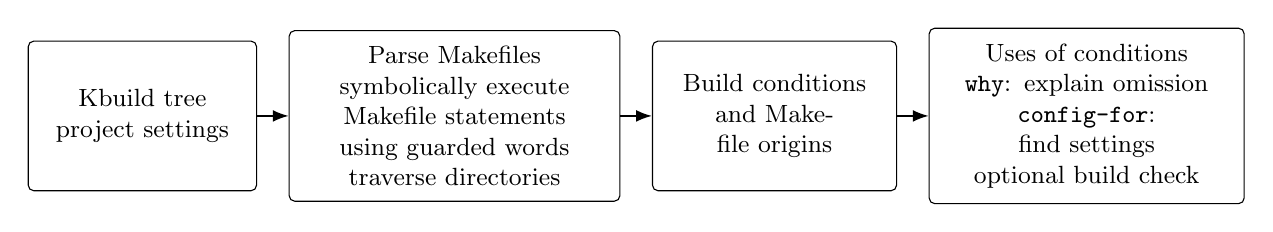
\begin{tikzpicture}[>=Latex,node distance=4mm,
  stage/.style={draw=black,rounded corners=2pt,align=center,inner sep=2mm,minimum height=19mm,font=\small}]
\node[stage,text width=25mm] (input) {Kbuild tree\\project settings};
\node[stage,text width=38mm,right=of input] (analysis) {Parse Makefiles\\symbolically execute\\Makefile statements\\using guarded words\\traverse directories};
\node[stage,text width=27mm,right=of analysis] (map) {Build conditions\\and Makefile origins};
\node[stage,text width=36mm,right=of map] (queries) {Uses of conditions\\\texttt{why}: explain omission\\\texttt{config-for}: find settings\\optional build check};
\draw[->,line width=0.6pt] (input)--(analysis);
\draw[->,line width=0.6pt] (analysis)--(map);
\draw[->,line width=0.6pt] (map)--(queries);
\end{tikzpicture}}
\caption{\tool evaluates Kbuild rules to obtain reusable build conditions and origins.
The rightmost box shows optional downstream queries: \texttt{why} explains a build verdict, while \texttt{config-for} proposes a configuration for selected files; a build can check the proposal.}
\Description{A compact left-to-right flow from a Kbuild tree and project settings through symbolic execution over guarded words to build conditions and Makefile origins, then to optional why and config-for queries with an optional build check.}
\label{fig:overview-pipeline}
\end{figure}

Given a source tree containing the Makefile in Figure~\ref{fig:kbuild-example}, \tool derives the built-in and module conditions in Table~\ref{tab:overview-conditions}.
The Makefile uses option and object names from Linux 6.6 \texttt{fs/ext4/Makefile}, with a constructed overwrite and branch to expose the analysis.
Both EXT4 options are tristate, so each can be \texttt{y}, \texttt{m}, or disabled.
In a generated Makefile, disabled \texttt{n} expands to an empty value and contributes to neither \texttt{obj-y} nor \texttt{obj-m}.
Write $E_y$ and $E_m$ for the two enabled values of \texttt{CONFIG\_EXT4\_FS}, and $T_y$ and $T_m$ for those of \texttt{CONFIG\_EXT4\_KUNIT\_TESTS}.
\texttt{CONFIG\_FS\_VERITY} is Boolean, so $V$ means it is \texttt{y} and $\neg V$ means it is disabled.
Kconfig also defines string, integer, and hexadecimal symbols, although this example uses none of them.

% Source names: results/workspaces/linux/fs/ext4/Makefile (Linux 6.6).
% The conditional overwrite and EXTRA branch below are illustrative changes.
\begin{figure}[t]
\centering
\begin{minipage}[t]{0.48\linewidth}
\vspace{0pt}
\begin{lstlisting}[style=kbuild-example]
# Adapted from Linux 6.6 fs/ext4/Makefile
obj-$(CONFIG_EXT4_FS) += ext4.o
obj-$(CONFIG_EXT4_KUNIT_TESTS) := ext4-inode-test.o
ifeq ($(CONFIG_FS_VERITY),y)
  EXTRA := verity
else
  EXTRA := crypto
endif
obj-y += $(EXTRA).o
ext4-inode-test-y += inode-test.o
\end{lstlisting}
\captionof{figure}{Input Makefile for the \tool walkthrough, adapted from Linux 6.6 \texttt{fs/ext4/Makefile}.
The overwrite and \texttt{EXTRA} branch are constructed for this walkthrough and are not verbatim Linux build rules.}
\Description{An adapted Kbuild Makefile with assignments to option-dependent obj variables, a conditional choosing between verity and crypto, an append to obj-y, and an inode-test member of a composite object.}
\label{fig:kbuild-example}
\end{minipage}\hfill
\begin{minipage}[t]{0.48\linewidth}
\vspace{0pt}
\captionof{table}{Local build conditions for Figure~\ref{fig:kbuild-example} before directory guards are applied.
The columns distinguish selection through \texttt{obj-y} and \texttt{obj-m}.}
\label{tab:overview-conditions}
\vspace{6pt}
\centering\small
\begin{tabular}{@{}lll@{}}
\toprule
Target or member & Built-in & Module \\
\midrule
\texttt{ext4.o} & $E_y\land\neg T_y$ & $E_m\land\neg T_m$ \\
\texttt{ext4-inode-test.o} & $T_y$ & $T_m$ \\
\texttt{inode-test.o} & $T_y$ & $T_m$ \\
\texttt{verity.o} & $V$ & --- \\
\texttt{crypto.o} & $\neg V$ & --- \\
\bottomrule
\end{tabular}
\end{minipage}
\end{figure}

\tool expands the first assignment destination to \texttt{obj-y} under $E_y$ and \texttt{obj-m} under $E_m$, adding \texttt{ext4.o} to the corresponding list.
The second assignment replaces \texttt{obj-y} under $T_y$ and \texttt{obj-m} under $T_m$, leaving the other list intact in each case.
Thus \texttt{ext4.o} survives as built-in under $E_y\land\neg T_y$ and as a module under $E_m\land\neg T_m$.
The condition for \texttt{ext4.o} depends on an assignment that does not name it.

Next, \tool evaluates both arms of the conditional and merges \texttt{EXTRA=verity} under $V$ with \texttt{EXTRA=crypto} under $\neg V$.
Expanding \texttt{\$(EXTRA).o} adds \texttt{verity.o} or \texttt{crypto.o} to \texttt{obj-y}, so this assignment has no module route.
\tool records \texttt{inode-test.o} as a member of \texttt{ext4-inode-test.o}.
The member follows its parent's built-in or module selection.

Table~\ref{tab:overview-conditions} describes target-list selection and composite membership within this Makefile.
A selected built-in composite does not necessarily produce a separate object file named after its parent.
For a nested Makefile, \tool then conjoins built-in selections with the guard $B$ for reaching the directory through a built-in route and module selections with the directory reachability guard $D$.
For example, \texttt{ext4.o} has the built-in condition $B\land E_y\land\neg T_y$ and the module condition $D\land E_m\land\neg T_m$.
Either route can select the object, so its overall build condition is $(B\land E_y\land\neg T_y)\lor(D\land E_m\land\neg T_m)$.
\tool also joins conditions with $\lor$ when separate Makefile assignments or directory paths select the same object.
These formulas describe the supported Kbuild analysis, while Kconfig feasibility and physical compilation are checked separately.

These build conditions support the two queries in Figure~\ref{fig:overview-pipeline}.
Given a \texttt{.config}, \tool's \texttt{why} command evaluates an object\textquotesingle s build condition and identifies the first failed part of its condition chain.
For example, if $B$, $E_y$, and $T_y$ hold, \texttt{why} reports that \texttt{ext4.o} is not selected because the later assignment replaced its \texttt{obj-y} entry.
The adapted example does not model Kconfig constraints, so this verdict concerns only its Makefile selection.



Given changed \texttt{.c} or \texttt{.S} files, or a patch, \tool's \texttt{config-for} command maps the touched source files to objects.
\tool combines their build conditions with the relevant Kconfig constraints and seeks a configuration close to a supplied base configuration.
It returns a fragment of option changes and reports files it cannot map or select together.
% Evidence: evidence/config_for_checkpoint_2b.json, synthetic_multi_file_sets and real_compile_spot_checks.
In a recorded Linux task, selecting \texttt{fs/btrfs/inode.o} from the saved base configuration required \texttt{CONFIG\_BTRFS\_FS=y}, and the proposed configuration survived \texttt{make olddefconfig} and compiled that object.
This Linux task supplies the Kconfig and build checks that the adapted Makefile cannot illustrate.

Applying the fragment through \texttt{make olddefconfig} checks whether the configurator preserves the requested values.
Compiling the selected object checks whether the proposed settings reach a physical build in that task.
A satisfying build condition alone establishes neither result, so \tool reports the proposal and its verification separately.
The next section explains how guarded execution and conditional directory traversal produce the map from object paths to build conditions.

\section{Technique}\label{sec:technique}

This section describes how \tool extracts reusable build conditions from Kbuild Makefiles and uses them to answer developer queries.
We first formalize the analysis setting and state the two core algorithms.
The remaining subsections explain include splicing, guarded assignments, branch merging, directory reachability, physical build semantics, and query evaluation.

\subsection{Setting and Problem Formulation}\label{sec:technique:setting}

Let $M$ denote the set of Kbuild Makefiles across a source repository, and let $c$ denote a configuration that assigns values to configuration options $\mathcal{O}$.
Each option in $\mathcal{O}$ is Boolean ($\texttt{y}$ or unset), tristate ($\texttt{y}$, $\texttt{m}$, or unset), or valued (string, integer, or hexadecimal).
We encode a Boolean or tristate option as one propositional variable per enabled value (e.g., $E_y$ and $E_m$, at most one true), and a Make test that compares a valued option with a literal as an atomic proposition over that option.
For an object path $o$, let $S_M(o, c)$ hold when the build system compiles $o$ under configuration $c$.
\tool computes a propositional formula $\Phi_M(o)$ over option variables such that evaluating $\Phi_M(o)$ under $c$ predicts $S_M(o, c)$.

To compute these formulas without enumerating configurations, \tool represents the value of each Make variable as a mapping from whitespace-separated words to build conditions.
(Variability and software product line literature often refers to configuration formulas guarding code or assets as presence conditions~\cite{liebig2010analysis,thum2014potential,berger2013variability,apel2013feature}.)
Throughout this paper, we consistently use the term \emph{build condition} to denote the propositional formula over configuration options under which a Make variable word, directory route, or compiled object file is selected.
Formally, an execution state $\sigma$ maps each variable name $n$ to a guarded word set $\sigma[n] = \{w \mapsto \phi_w\}$, where $\phi_w$ is a propositional build condition denoting when word $w$ belongs to variable $n$.
We write $\sigma[n](w) = \bot$ when word $w$ is absent from variable $n$.
For two guarded word sets, $\sigma_1[n] \sqcup \sigma_2[n]$ denotes their pointwise disjunction, where the build condition of each word $w$ becomes $\sigma_1[n](w) \lor \sigma_2[n](w)$.

\begin{algorithm}[t]
\caption{Extract guarded Kbuild object conditions}
\label{alg:extract}
\begin{algorithmic}[1]
\Require Source tree $M$, guarded entry files $E$, project settings $\Gamma$
\Ensure Map $\Phi$ from object paths to build conditions and origins
\State $R[m] \gets \bot$ for each file $m \in M$; $Q \gets E$
\State $C \gets \text{empty map}$; $I \gets \emptyset$
\While{$Q$ is nonempty}
  \State remove $(m, \gamma)$ from $Q$
  \State $\delta \gets \gamma \land \neg R[m]$
  \If{$\delta$ is unsatisfiable}
    \State \textbf{continue}
  \EndIf
  \If{$C[m]$ is undefined}
    \State $C[m] \gets \textsc{Exec}(\operatorname{reduce}(\operatorname{splice}(\operatorname{parse}(m))), \sigma_\Gamma, \top)$
  \EndIf
  \State $S \gets \operatorname{restrict}(C[m], \delta)$
  \State $R[m] \gets R[m] \lor \gamma$; add $S$ to $I$
  \For{each selected directory $(d, \eta)$ in $S$}
    \State add $(\operatorname{entry}(d), \eta)$ to $Q$ if its entry file exists
  \EndFor
\EndWhile
\State $\Phi \gets \emptyset$
\For{each restricted instance $S \in I$}
  \For{each target, member, or program object $(o, \phi) \in \operatorname{objects}(S, \Gamma)$}
    \State $\Phi[o] \gets \Phi[o] \lor \phi$ \Comment{initially $\bot$}
  \EndFor
\EndFor
\State $\Phi \gets \operatorname{close}(\Phi, I, \Gamma)$ \Comment{resolve composite members, built-in routes, and rules}
\State \Return $\Phi$
\end{algorithmic}
\end{algorithm}

Algorithm~\ref{alg:extract} presents the end-to-end extraction procedure.
Lines 1--2 initialize the worklist $Q$ with the configured entry files and set the accumulated reachability guard $R[m]$ for every file to false.
Lines 3--17 process reachable Makefiles along incoming directory paths.
For each work item $(m, \gamma)$, line 5 computes the incremental guard $\delta = \gamma \land \neg R[m]$ that has not yet been explored for $m$.
If $\delta$ is unsatisfiable, lines 6--8 discard the item.
Otherwise, lines 9--11 execute the parsed and spliced Makefile under an unrestricted guard when encountering $m$ for the first time, caching the result in $C[m]$.
Line 12 restricts the cached state $C[m]$ to the active guard $\delta$, producing an analyzed instance $S$, and line 13 records $S$ and updates $R[m]$.
Lines 14--16 extract downstream directories selected in $S$ and queue their entry Makefiles under their respective directory guards $\eta$.
After the traversal terminates, lines 18--23 aggregate target words across all recorded instances.
Finally, line 24 computes the transitive closure over composite members, built-in directory reachability constraints, and rule prerequisites before returning the completed map $\Phi$.

\begin{algorithm}[t]
\caption{\textsc{Exec}: execute one statement over guarded words}
\label{alg:exec}
\begin{algorithmic}[1]
\Require Statement $s$, state $\sigma$, ambient guard $g$
\Ensure Updated state $\sigma$
\If{$s$ is an assignment $x\ \mathit{op}\ e$}
  \State $V \gets \{w \mapsto \phi_w\}$ from $\operatorname{expand}(e, \sigma)$, or $\{e \mapsto \top\}$ if $\mathit{op}$ defers $e$ and $e$ contains a reference
  \For{each guarded variable name $(n, \psi_n) \in \operatorname{expand}(x, \sigma)$}
    \State $\psi \gets g \land \psi_n$
    \If{$\mathit{op} \in \{\texttt{=}, \texttt{:=}\}$ or $\sigma[n]$ is undefined}
      \State $\sigma[n] \gets \{w \mapsto \psi \land \phi_w\} \sqcup \{w \mapsto \phi \land \neg\psi : (w \mapsto \phi) \in \sigma[n]\}$
    \Else \Comment{$\mathit{op} = \texttt{+=}$}
      \State $\sigma[n] \gets \sigma[n] \sqcup \{w \mapsto \psi \land \phi_w\}$
    \EndIf
  \EndFor
\ElsIf{$s$ is a conditional with test $t$, then-arm $T$, else-arm $F$}
  \State $\kappa \gets \operatorname{cond}(t, \sigma)$; $\sigma_t \gets \text{copy of } \sigma$; $\sigma_e \gets \text{copy of } \sigma$
  \State $\textsc{Exec}(T, \sigma_t, g \land \kappa)$; $\textsc{Exec}(F, \sigma_e, g \land \neg\kappa)$
  \For{each variable name $n$ assigned in $T$ or $F$}
    \If{$\sigma_t[n](w) = \sigma_e[n](w) = \phi$}
      \State $\sigma[n](w) \gets g \land \phi$ \Comment{fast-path merge for untouched words}
    \Else
      \State $\sigma[n](w) \gets (g \land \kappa \land \sigma_t[n](w)) \lor (g \land \neg\kappa \land \sigma_e[n](w))$
    \EndIf
  \EndFor
\EndIf
\State \Return $\sigma$
\end{algorithmic}
\end{algorithm}

Algorithm~\ref{alg:exec} defines the symbolic execution routine \textsc{Exec} for individual Make statements.
Lines 1--10 handle variable assignments by expanding both the destination variable name and the assigned expression into guarded words.
Lines 11--20 handle conditionals by evaluating the test condition, executing both branches on separate copies of the state, and merging modified variables back into $\sigma$.
We now examine each stage of this analysis in detail.

\subsection{Parsing, Include Splicing, and Dependency Reduction}\label{sec:technique:include}

\tool reads each Makefile and parses its syntax with \texttt{pymake3}.
In Kbuild, an \texttt{include} directive evaluates a referenced file within the environment of the including Makefile, using the repository root as its working directory.
\tool mirrors this behavior through \emph{static include splicing}: it resolves the path of each included file and substitutes the directive with the parsed statements of the target file before running symbolic execution.
Path resolution evaluates standard Kbuild variables such as \texttt{src}, \texttt{obj}, and \texttt{srctree}, as well as constant assignments and string functions such as \texttt{addprefix} and \texttt{addsuffix}.
For example, the Linux AMD GPU driver defines \texttt{FULL\_AMD\_PATH := \$(srctree)/\$(src)/..} and uses \texttt{addprefix} to include 51 display-library Makefiles.
\tool resolves 742 composite-member objects under \path{drivers/gpu/drm/amd/}; without splicing it finds only 240 of them.
When an include path depends on dynamic shell outputs or unresolvable variables, \tool records the unmerged include and continues analysis.

After splicing includes, \tool performs static dependency reduction.
Many statements in Kbuild Makefiles manipulate compiler flags (such as \texttt{ccflags-y} and \texttt{CFLAGS}) that do not affect which object files are selected.
\tool computes the backward dependency cone of all target-affecting variables, composite lists, subdirectories, and build rules.
It then removes statements that do not influence these variables before invoking \textsc{Exec}.
This reduction discards irrelevant flag manipulations, keeping subsequent symbolic execution focused on target selection.

\subsection{Guarded Assignment and Name Expansion}\label{sec:technique:assign}

Kbuild Makefiles construct target lists by appending and assigning to variables whose names and values contain option references.
Algorithm~\ref{alg:exec} evaluates an assignment $x\ \mathit{op}\ e$ by expanding the left-hand name $x$ into a set of guarded variable names $\{(n, \psi_n)\}$ and the right-hand expression $e$ into a set of guarded words $\{(w, \phi_w)\}$.
The effective guard for writing word $w$ into variable $n$ is $\psi = g \land \psi_n \land \phi_w$, where $g$ is the ambient execution guard.

When an assignment appends to a variable ($\mathit{op} = \texttt{+=}$), line 8 joins the new guarded words into $\sigma[n]$ using pointwise disjunction $\sqcup$.
When an assignment overwrites a variable ($\mathit{op} \in \{\texttt{=}, \texttt{:=}\}$), line 6 updates the state conditionally.
The assigned words receive the active guard $\psi \land \phi_w$.
Crucially, any pre-existing word $(w \mapsto \phi)$ in $\sigma[n]$ survives under the narrowed condition $\phi \land \neg\psi$, reflecting that the overwrite replaced the previous definition only in configurations where $\psi$ holds.
A conditional default (\texttt{?=}) leaves existing words untouched and adds each new word under $\psi \land \phi_w \land \neg\bigvee_{w'} \sigma[n](w')$, that is, only where the variable holds no words; Algorithm~\ref{alg:exec} omits this case for brevity.

Consider the following pair of Kbuild assignments:
\begin{lstlisting}[style=kbuild-example]
obj-$(CONFIG_A) += a.o
obj-$(CONFIG_B) := b.o
\end{lstlisting}
Assuming an initially empty state $\sigma[\texttt{obj-y}] = \emptyset$, line 1 expands the destination to \texttt{obj-y} under $A_y = (\texttt{CONFIG\_A=y})$.
Appending \texttt{a.o} yields $\sigma[\texttt{obj-y}] = \{\texttt{a.o} \mapsto A_y\}$.
Line 2 then expands its destination to \texttt{obj-y} under $B_y = (\texttt{CONFIG\_B=y})$.
Because line 2 is an overwrite (\texttt{:=}), \tool assigns \texttt{b.o} under $B_y$ and narrows the existing entry \texttt{a.o} by $\neg B_y$, producing the updated state $\sigma[\texttt{obj-y}] = \{\texttt{a.o} \mapsto A_y \land \neg B_y,\ \texttt{b.o} \mapsto B_y\}$.
The build condition of \texttt{a.o} accurately captures that \texttt{b.o} replaces it whenever $B_y$ holds.

\begin{table}[t]
\centering\footnotesize
\caption{Kbuild Make constructs and \tool's modeled semantics.}
\label{tab:make-scope}
\begin{tabular}{p{28mm}p{48mm}p{48mm}}
\toprule
Construct & Modeled Semantics & Boundary \\
\midrule
\texttt{+=}, \texttt{=}, \texttt{:=}, \texttt{::=} & Guarded words; GNU Make flavor handling (\texttt{::=} as \texttt{:=}); deferred target lists expanded at file end & Word ordering and duplicate occurrences are not preserved. \\
\texttt{?=} & Assigned under the configurations in which the variable holds no words & Differs from GNU Make when a variable is defined but empty. \\
\texttt{ifeq}, \texttt{ifneq}, \texttt{ifdef}, \texttt{ifndef} & Evaluates condition guard, executes both arms on copies, merges modified variables & Tests inherit the limits of variable references below. \\
Variable references & Guarded words plus empty string alternative; substitution references per word & Concatenation collapses when alternatives exceed 64 combinations. \\
Text functions & Handled symbolically for \texttt{filter}, \texttt{patsubst}, \texttt{addprefix}, \texttt{addsuffix}, \texttt{word} & Arbitrary custom recursive functions are unrolled to a fixed depth. \\
\texttt{include} & Recursively spliced when target path resolves statically & Unresolved dynamic include paths contribute no statements. \\
Rules and sub-makes & Targets and prerequisites captured as guarded lists; followed to closure & Recipes other than sub-makes are not executed. \\
\texttt{\$(shell ...)} & Executed as concrete subprocess with timeout; empty in sandbox mode & Output reflects the host environment and installed tools. \\
\bottomrule
\end{tabular}
\end{table}

\tool models GNU Make variable expansion flavors.
For simply expanded assignments (\texttt{:=}), \tool expands the right-hand expression immediately during execution.
For recursively expanded assignments (\texttt{=}) and conditional defaults (\texttt{?=}), \tool stores unexpanded expression text containing variable references and defers evaluation until the end of the Makefile.
This deferred expansion matches Kbuild semantics, because Kbuild reads final target variables only after processing the complete file.
For example, in Linux's \texttt{drivers/xen/Makefile}, the assignment \texttt{dom0-y += \$(xen-pad-y)} precedes the definition of \texttt{xen-pad-y}; deferred evaluation correctly resolves the reference to include \texttt{xen-acpi-pad.o}.
Table~\ref{tab:make-scope} summarizes the supported Make constructs and their operational boundaries.

\subsection{Conditional Execution and Branch Merging}\label{sec:technique:merge}

Kbuild Makefiles make extensive use of conditional directives (\texttt{ifeq}, \texttt{ifneq}, \texttt{ifdef}, and \texttt{ifndef}).
When encountering a conditional statement, Algorithm~\ref{alg:exec} evaluates the test expression $t$ under the current state $\sigma$ to produce a guard formula $\kappa$.
For equality tests, \tool expands both sides into guarded strings and defines $\kappa$ as the disjunction of guards where the two sides coincide.
For example, testing \texttt{ifeq (\$(CONFIG\_FS\_VERITY),y)} produces $\kappa = V$.

Rather than forking the entire execution path into separate analysis branches, \tool creates copies of the state $\sigma_t$ and $\sigma_e$ for the then-arm and else-arm (line 12).
It executes the then-arm $T$ under ambient guard $g \land \kappa$ and the else-arm $F$ under $g \land \neg\kappa$ (line 13).
Lines 14--19 then merge modified variables back into $\sigma$.
For each variable $n$ assigned in either branch, an entry present with guard $\phi_t$ in the then-branch and $\phi_e$ in the else-branch receives the combined guard $(g \land \kappa \land \phi_t) \lor (g \land \neg\kappa \land \phi_e)$.
Conjoining the ambient guard $g$ is safe inside nested conditionals: the enclosing merge re-gates the whole arm with its own branch guard and restores the configurations outside $g$ from the other arm.

To illustrate the contrast between path forking and \tool's state folding, consider sequential conditionals:
\begin{lstlisting}[style=kbuild-example]
ifeq ($(CONFIG_A),y)
  obj-y += a.o
endif
ifeq ($(CONFIG_B),y)
  obj-y += b.o
endif
\end{lstlisting}
A classic path-forking symbolic executor forks at each conditional, maintaining $2^2 = 4$ separate path environments:
$\pi_1(A \land B) \mapsto \{\texttt{a.o}, \texttt{b.o}\}$, $\pi_2(A \land \neg B) \mapsto \{\texttt{a.o}\}$, $\pi_3(\neg A \land B) \mapsto \{\texttt{b.o}\}$, and $\pi_4(\neg A \land \neg B) \mapsto \emptyset$.
For $k$ sequential blocks, path forking produces $O(2^k)$ execution paths.

In contrast, \tool folds branch states at each \texttt{endif} in linear time.
After block 1, \tool holds the single folded state $\sigma[\texttt{obj-y}] = \{\texttt{a.o} \mapsto A\}$.
When evaluating block 2, the then-arm produces $\sigma_t[\texttt{obj-y}] = \{\texttt{a.o} \mapsto A, \texttt{b.o} \mapsto B\}$ under ambient guard $B$, while the else-arm produces $\sigma_e[\texttt{obj-y}] = \{\texttt{a.o} \mapsto A\}$ under $\neg B$.
At the join point, \tool observes that \texttt{a.o} carries the exact same guard $A$ in both arms ($\sigma_t[\texttt{obj-y}](\texttt{a.o}) = \sigma_e[\texttt{obj-y}](\texttt{a.o}) = A$).
Line 16 applies the fast-path merge, setting the guard of \texttt{a.o} directly to $g \land A = A$ (here $g = \top$) rather than creating the redundant disjunction $(B \land A) \lor (\neg B \land A)$.
The final state is $\{\texttt{a.o} \mapsto A,\ \texttt{b.o} \mapsto B\}$, computed in $O(k)$ linear time without path explosion.
The identity $(g \land \kappa \land \phi) \lor (g \land \neg\kappa \land \phi) \equiv g \land \phi$ makes this simplification exact.

\subsection{Conditional Directory Reachability}\label{sec:technique:worklist}

Kbuild orchestrates large source trees hierarchically: a parent Makefile descends into subdirectories listed in target variables and subdirectory lists (\texttt{obj-y}, \texttt{obj-m}, \texttt{subdir-y}, and \texttt{subdir-m}).
Algorithm~\ref{alg:extract} explores this directory structure using a worklist $Q$ starting from top-level entry files $E$.

A naive traversal using a Boolean visited set would fail when the same directory is reachable through multiple independent paths with different configuration guards.
Conversely, re-executing a Makefile on every visit would lead to redundant work.
\tool resolves this trade-off by maintaining an accumulated reachability guard $R[m]$ for each Makefile $m$.
When a work item $(m, \gamma)$ is dequeued, line 5 computes the uncovered guard $\delta = \gamma \land \neg R[m]$.
If Z3 determines that $\delta$ is unsatisfiable, the visit is redundant and skipped.
Otherwise, lines 9--11 obtain the cached baseline execution state $C[m]$ and line 12 restricts it by conjoining all guards with $\delta$.
Line 13 updates $R[m] \gets R[m] \lor \gamma$.
Lines 14--16 then extract directory targets and append child Makefiles to $Q$ alongside their reachability guards $\eta$.

Consider a top-level Makefile that reaches a subdirectory through two independent option routes:
\begin{lstlisting}[style=kbuild-example]
obj-$(CONFIG_NET) += drivers/net/
obj-$(CONFIG_PCI) += drivers/net/
\end{lstlisting}
When processing the first entry under guard $N$ (for \texttt{CONFIG\_NET=y}), \tool executes \path{drivers/net/Makefile} once under $\top$, caches its execution state $C[\texttt{net}]$, restricts it to $N$, and records $R[\texttt{net}] = N$.
When the second entry arrives under guard $P$ (for \texttt{CONFIG\_PCI=y}), \tool computes $\delta = P \land \neg N$.
If Z3 determines that $\delta$ is satisfiable, \tool restricts the cached state $C[\texttt{net}]$ by $\delta$, updates $R[\texttt{net}] = N \lor P$, and queues newly reachable subdirectories.
If $P$ already implies $N$, $\delta$ is unsatisfiable and \tool skips the visit entirely.
Because the source repository contains a finite number of Makefiles and option domains are finite, $R[m]$ can strictly weaken only finitely many times, guaranteeing termination.

\subsection{Object Extraction and Kbuild Build Semantics}\label{sec:technique:build}

After the directory worklist terminates, \tool extracts physical object paths from the recorded instances $I$.
Target extraction inspects standard Kbuild target families (\texttt{obj-}, \texttt{lib-}, \texttt{extra-}, and \texttt{always-}) as well as project-specific families (such as \texttt{pbl-} in Barebox and \texttt{bootblock-} in coreboot).
\tool models four core build semantics from Kbuild's \texttt{scripts/Makefile.build}:

\paragraph{Composite Object Resolution.}
When a selected target $t$ represents a composite object, Kbuild compiles its constituent members rather than a single source file of the same name.
\tool inspects composite definitions in variables such as \texttt{$t$-y}, \texttt{$t$-objs}, \texttt{$t$-lib}, and \texttt{$t$-m}.
It assigns each member object the conjunction of its own guard and the container object's guard.
In Linux v6.6, composite members account for 14,351 of the 29,245 analyzed object paths.

\paragraph{Built-in Containers and Objects.}
When a composite target is selected for a built-in build (\texttt{obj-y}), Kbuild links its member objects directly into the directory's archive (\texttt{built-in.a}) and produces no standalone object file for the container name.
Only module composites (\texttt{obj-m}) generate container object files on disk.
\tool therefore suppresses built-in composite container paths from the final object map while preserving their member objects.

\paragraph{Built-in Directory Reachability Routes.}
Kbuild sets an internal flag \texttt{need-builtin} during recursive builds: a directory builds its \texttt{built-in.a} archive and its \texttt{obj-y} targets only if the parent directory was entered through an \texttt{obj-y} reference.
If a directory is reached solely through an \texttt{obj-m} or \texttt{subdir-y} reference, Kbuild builds its modules and auxiliary targets but skips its \texttt{obj-y} objects.
\tool computes the built-in reachability guard $B_m$ for every Makefile $m$ as a fixpoint over \texttt{obj-y} directory edges and conjoins $B_m$ with every built-in object guard.

\paragraph{Rule Prerequisites and Sub-makes.}
Certain kernel objects do not appear in target lists and are built only when invoked as prerequisites of explicit or pattern rules.
For example, vDSO objects and boot images are compiled through architecture-specific rules in \texttt{arch/x86/entry/vdso/Makefile} and \texttt{arch/x86/boot/Makefile}.
\tool records explicit rules, pattern rules, and sub-make invocations of the form \texttt{\$(MAKE) \$(build)=\textit{dir} \textit{goal}} as guarded structures.
Line 24 of Algorithm~\ref{alg:extract} computes a prerequisite closure starting from all selected objects and configured goals, pulling in rule prerequisites under the conjunction of their triggering guards.

\subsection{Applications: Developer Queries and Analysis Cache}\label{sec:technique:queries}

The resulting map $\Phi$ stores the exact build conditions and origin Makefiles for all discovered objects.
\tool uses this map to answer developer queries about the project build without re-analyzing the source tree. 

\paragraph{Explaining Omissions (\texttt{why}).}
Given a configuration file \texttt{.config} and a target object path $o$, \tool evaluates $\Phi(o)$ under the supplied configuration.
If the condition evaluates to false, \tool traverses the chain of conditions that produced $\Phi(o)$---including directory reachability, assignment guards, and composite membership---and identifies the first unsatisfied guard term.
This pinpoints whether the object was omitted due to an unset top-level option, a directory bypass, or an overwrite in a specific Makefile.

\paragraph{Enabling Changed Files (\texttt{config-for}).}
Given a set of modified source files or a patch, \tool maps each source file to its corresponding object path $o$ and retrieves build condition $\Phi(o)$.
To ensure that the requested options can be enabled without violating kernel dependencies, \tool extracts the Kconfig dependency cone for all options appearing in $\Phi(o)$.
It translates both the build conditions and the Kconfig dependencies into a propositional formula and queries Z3 to find a satisfying assignment that minimizes changes relative to a base \texttt{.config}.
If the targets have conflicting requirements, \tool reports the mutually incompatible file subsets.

\paragraph{Analysis Cache and Invalidation.}
\tool persists each object's kind, origins, and build condition, together with the reachability conditions of analyzed Makefiles, in a per-tree cache: a JSON metadata file plus the conditions as SMT-LIB terms with shared subterms.
Subsequent invocations of \texttt{why} and \texttt{config-for} load this cache and parse conditions lazily, one object at a time.
The cache records the path, modification time, and size of every Makefile, included fragment, and settings file the analysis read, plus a content hash of the analyzer itself.
If any of these changes, \tool discards the cache and reruns the whole-tree analysis; incremental re-analysis is future work.

\section{Evaluation}\label{sec:evaluation}

This section evaluates \tool across five configurable software projects: the Linux kernel (v6.6), BusyBox (1.36.1), Barebox (2024.01.0), Das U-Boot (2024.01), and coreboot (4.22.01).
Our evaluation investigates four research questions:
\begin{itemize}
\tightlist
\item \textbf{RQ1 (Build Agreement):} How accurately do \tool's extracted build conditions predict compiled object files across concrete configurations and diverse Kbuild dialects? (\S\ref{sec:eval:agreement})
\item \textbf{RQ2 (Scalability and State Folding):} Does state-folding symbolic execution avoid the state explosion of path-forking symbolic execution, and how fast is whole-tree analysis? (\S\ref{sec:eval:scaling})
\item \textbf{RQ3 (Developer Diagnostics and Automated Configuration):} How effectively do \tool's \texttt{why} and \texttt{config-for} queries explain build omissions and synthesize configuration fragments for modified source code? (\S\ref{sec:eval:developer})
\item \textbf{RQ4 (Comparative Analysis and Ablations):} How does \tool compare with \kmax on the same physical builds, and which Kbuild modeling features account for its agreement? (\S\ref{sec:eval:comparative})
\end{itemize}

\subsection{Experimental Setup and Provenance}\label{sec:eval:setup}

Table~\ref{tab:subjects} summarizes the evaluated subjects, their tested configurations, and their physical artifact status.
For Linux, we evaluate four x86 configurations spanning minimal to exhaustive profiles: i386 \texttt{tinyconfig} (489 compiled objects), x86-64 \texttt{defconfig} (2,874 compiled objects), Debian x86-64 distribution configuration (15,419 compiled objects), and x86-64 \texttt{allmodconfig} (25,949 compiled objects).
Clean rebuilds using GCC 12.5.0 reproduced the exact physical object inventories for Linux \texttt{tinyconfig}, Linux \texttt{defconfig}, and Barebox \texttt{sandbox\_defconfig}.
The Debian and \texttt{allmodconfig} Linux comparisons, BusyBox, coreboot, and one U-Boot comparison use archived build inventories; a second, fresh U-Boot build completed compilation but failed during final packaging.
The Linux archives omit \texttt{tools/} and \texttt{scripts/}; predictions under top-level directories absent from an archive are reported separately rather than counted as false positives (one object, under \texttt{allmodconfig}).

All experiments were executed on an Intel Core i7-7700 workstation equipped with 8 logical CPUs and 31\,GiB of RAM running Debian Linux.
The analysis environment ran Python 3.14.7, Z3 4.13.3, and GNU Make 4.4.1.
Exact source repository commits and configuration SHA-256 hashes are recorded in \texttt{evidence/manifest.json}.
% Canonical run for RQ1, RQ2 timing, and RQ4 ablations: results/physical_validation.json and results/ablation.json (2026-09-25).
% The older results/*_20260924.json files predate composite-member resolution and are superseded.

\begin{table}[t]
\centering\footnotesize
\caption{Evaluated subject systems, configurations, and build provenance.}
\label{tab:subjects}
\begin{tabular}{lllr}
\toprule
Subject & Version / Commit & Tested Configuration & Physical Objects \\
\midrule
Linux & v6.6 (\texttt{ffc25326}) & i386 \texttt{tinyconfig} & 489 \\
Linux & v6.6 (\texttt{ffc25326}) & x86-64 \texttt{defconfig} & 2,874 \\
Linux & v6.6 (\texttt{ffc25326}) & Debian x86-64 & 15,419 \\
Linux & v6.6 (\texttt{ffc25326}) & x86-64 \texttt{allmodconfig} & 25,949 \\
Barebox & 2024.01.0 & \texttt{sandbox\_defconfig} & 406 \\
Das U-Boot & 2024.01 & \texttt{sandbox\_defconfig} (archived / fresh) & 1,123 / 1,309 \\
BusyBox & 1.36.1 & \texttt{defconfig} & 191 \\
coreboot & 4.22.01 & QEMU i440fx & 674 \\
\bottomrule
\end{tabular}
\end{table}

\subsection{RQ1: Build Agreement}\label{sec:eval:agreement}

To evaluate agreement, we compare \tool's predicted object sets against concrete physical build outputs.
Let $U$ denote the set of extracted object paths (targets, composite members, programs, and rule prerequisites), and let $P_c \subseteq U$ denote the predicted object set obtained by evaluating all build conditions under configuration $c$.
Let $B_c$ denote the ground-truth inventory of physical \texttt{.o} files compiled on disk under $c$.
We partition the comparison into true positives $TP = |P_c \cap B_c|$, false positives $FP = |P_c \setminus B_c|$, misses within the extracted set $FN_U = |(B_c \cap U) \setminus P_c|$, and physical objects outside the extracted set $O = |B_c \setminus U|$.
Precision is defined as $TP / (TP + FP)$, while whole-inventory overlap is defined as $TP / |B_c|$.

\begin{table}[t]
\centering\footnotesize
\caption{Linux physical build agreement across four configuration profiles.
The last column gives overlap when composite members are not resolved (targets only).}
\label{tab:linux-physical}
\begin{tabular}{lrrrrrrrr}
\toprule
Configuration & Pred. ($|P_c|$) & $TP$ & $FP$ & $FN_U$ & $O$ & Prec. & Overlap & Targets only \\
\midrule
\texttt{tinyconfig} (i386) & 489 & 489 & 0 & 0 & 0 & 100\% & 100\% & 88.5\% \\
\texttt{defconfig} (x86-64) & 2,874 & 2,874 & 0 & 0 & 0 & 100\% & 100\% & 49.4\% \\
Debian (x86-64) & 15,419 & 15,419 & 0 & 0 & 0 & 100\% & 100\% & 38.2\% \\
\texttt{allmodconfig} (x86-64) & 25,949 & 25,949 & 0 & 0 & 0 & 100\% & 100\% & 47.4\% \\
\bottomrule
\end{tabular}
\end{table}

Table~\ref{tab:linux-physical} reports the physical build comparison for Linux v6.6.
On all four profiles, the predicted set equals the physical \texttt{.o} inventory: every compiled object is predicted and every predicted object is compiled.
The extracted set $U$ holds 29,245 object paths, of which 24,596--29,233 fall inside the top-level directories each archive covers.
Composite members are essential to this result.
Counting only the words of target-family variables, \tool's predictions cover 38.2--88.5\% of each inventory, because most compiled objects of built-in and module composites never appear in a target list themselves.

\begin{table}[t]
\centering\footnotesize
\caption{Physical build agreement for the four non-Linux subjects.}
\label{tab:firmware-physical}
\begin{tabular}{lrrrrrrr}
\toprule
Subject & Pred. ($|P_c|$) & $TP$ & $FP$ & $FN_U$ & $O$ & Prec. & Overlap \\
\midrule
BusyBox & 162 & 162 & 0 & 0 & 29 & 100.0\% & 84.8\% \\
Barebox & 406 & 402 & 4 & 0 & 4 & 99.0\% & 99.0\% \\
Das U-Boot (archived) & 1,029 & 952 & 77 & 0 & 171 & 92.5\% & 84.8\% \\
Das U-Boot (fresh) & 1,029 & 1,029 & 0 & 0 & 280 & 100.0\% & 78.6\% \\
coreboot & 540 & 437 & 103 & 0 & 237 & 80.9\% & 64.8\% \\
\bottomrule
\end{tabular}
\end{table}

Table~\ref{tab:firmware-physical} presents physical agreement across the four other projects.
No subject has a miss inside the extracted set.
On BusyBox, \tool achieves 100\% precision ($162/162$); all 29 outside objects are intermediate \texttt{built-in.o} archives, which older Kbuild dialects produce as \texttt{.o} files.
On Barebox, precision and overlap are both 99.0\%; the four outside objects are generated image metadata and embedded default-environment blobs.
On U-Boot, the 77 false positives against the archived build (41 under \texttt{lib/} and 36 under \texttt{cmd/}) disappear against the fresh build, which suggests that the archived inventory and configuration are out of step; most outside objects are driver objects (121) selected outside the analyzed Makefile traversal, and the fresh build adds host tools and generated files.
On coreboot, precision is 80.9\%: all 103 false positives lie under the stage-specific build directories \texttt{verstage}, \texttt{smm}, and \texttt{decompressor}, reflecting coreboot's multi-stage compilation model, and most outside objects are host utilities (\texttt{build/util}) and external payloads.
% TODO: confirm the U-Boot archive/config mismatch explanation by diffing the archived and fresh .config files.

\subsection{RQ2: Scalability and State Folding vs. Path Forking}\label{sec:eval:scaling}

To isolate the effect of state folding, we generated Makefiles with $k$ independent options in four families (\texttt{tools/bench\_scaling.py}):
\emph{append} (\texttt{obj-\$(CONFIG\_A$_i$) += a$_i$.o}),
\emph{ifeq} (an \texttt{ifeq} block that appends \texttt{b$_i$.o} to \texttt{obj-y}),
\emph{value} (an \texttt{ifeq}/\texttt{else} that sets \texttt{V$_i$}, followed by \texttt{obj-y += c$_i$\_\$(V$_i$).o}), and
\emph{indirect} (\texttt{ifeq} blocks that append \texttt{d$_i$.o} to an intermediate \texttt{OBJS}, followed by \texttt{obj-y += \$(OBJS)}).
We compare \tool with a path-forking executor built from the same code base (commit \texttt{a3c1683}) and with \kmax, under a five-minute timeout.

\begin{table}[t]
\centering\small
\caption{Scaling on generated Makefiles: path-forking states and seconds per family, and the slowest \tool and \kmax time over all four families.
All times include process start-up (about 0.5\,s).
``t/o'' marks the five-minute timeout and ``--'' a run skipped after a smaller $k$ timed out.}
\label{tab:scaling-bench}
\begin{tabular}{@{}rrrrrr@{}}
\toprule
& \multicolumn{3}{c}{Path forking: states / time (s)} & \tool & \kmax \\
\cmidrule(lr){2-4}
$k$ & \emph{ifeq} & \emph{value} & \emph{indirect} & time (s) & time (s) \\
\midrule
4 & 5 / 0.59 & 64 / 0.62 & 33 / 0.53 & 0.63 & 0.69 \\
8 & 9 / 0.71 & 2,048 / 3.18 & 1,025 / 0.86 & 0.63 & 0.69 \\
12 & 13 / 0.96 & 49,152 / 75.51 & 24,577 / 8.65 & 0.62 & 0.79 \\
16 & 17 / 1.50 & t/o & 524,289 / 184.59 & 0.62 & 0.70 \\
20 & 21 / 2.54 & -- & t/o & 0.63 & 0.71 \\
64 & 65 / 265.79 & -- & -- & 0.62 & 0.79 \\
128 & t/o & -- & -- & 0.73 & 0.90 \\
\bottomrule
\end{tabular}
\end{table}

Table~\ref{tab:scaling-bench} reports the results.
The path-forking executor's state count stays linear for \emph{append} (2$k$ states; 256 at $k=128$) and for \emph{ifeq} ($k+1$ states), because independent appends to the target list can be joined without enumerating combinations; its time on \emph{ifeq} still grows superlinearly and exceeds the timeout at $k=128$.
When branches write values that are later combined, forking explodes exponentially: \emph{indirect} reaches 524,289 states and 184.6\,s at $k=16$ and times out at $k=20$, and \emph{value} reaches 49,152 states at $k=12$ and times out at $k=16$.
\tool's time is flat at 0.61--0.73\,s for every family up to $k=128$ and dominated by start-up, and its object sets match the expected sets exactly in every run.
\kmax is also fast on all four families (0.67--0.90\,s), so this benchmark separates state folding from path forking, not \tool from \kmax.
On the \emph{value} family, \kmax reports $3k$ objects where $2k$ are expected.
% TODO: inspect the extra Kmax objects on the value family before characterizing them further.

\begin{table}[t]
\centering\small
\caption{End-to-end extraction performance on the five repositories (\texttt{results/physical\_validation.json}).}
\label{tab:corpus-timing}
\begin{tabular}{@{}lrrrrr@{}}
\toprule
Subject & Makefile instances & Targets & All objects & Time (s) & Peak RSS (MB) \\
\midrule
BusyBox & 29 & 609 & 609 & 0.27 & 65.6 \\
Barebox & 160 & 1,363 & 1,436 & 0.96 & 91.6 \\
Das U-Boot & 289 & 3,133 & 3,209 & 3.02 & 94.7 \\
coreboot & 458 & 4,594 & 4,594 & 7.98 & 90.5 \\
Linux x86 & 2,022 & 14,793 & 29,245 & 34.05 & 161.7 \\
\bottomrule
\end{tabular}
\end{table}

Table~\ref{tab:corpus-timing} reports end-to-end extraction runtime and object volume across all five repositories.
For the Linux x86 tree, \tool parses and symbolically executes 2,022 Makefile instances, issues 82,405 solver checks, and extracts build conditions for 29,245 object paths (14,793 target words plus composite members, programs, and rule prerequisites) in 34.05 seconds with 161.7\,MB of peak resident memory.
The four other repositories complete extraction in under 8 seconds.
Whole-tree analysis is therefore fast enough to run once per tree revision and reuse through the analysis cache, as the developer queries in RQ3 do.

\subsection{RQ3: Developer Diagnostics and Automated Configuration}\label{sec:eval:developer}

We evaluate \tool's developer-facing commands on Linux maintenance tasks.

\paragraph{Explaining Omissions (\texttt{why}).}
We evaluated \tool's \texttt{why} command on 28 object targets across Linux \texttt{defconfig} and \texttt{tinyconfig}.
For all 28 targets, \texttt{why} produced build verdicts matching the physical build inventories.
For excluded targets, \texttt{why} pinpointed the failed part of the condition chain, for example an unset top-level option (\texttt{CONFIG\_BTRFS\_FS} unset in \texttt{defconfig}) or an unsatisfied directory reachability route (\texttt{drivers/net/} not entered under \texttt{tinyconfig}).
% TODO: cite the evidence file for the 28 why cases and say whether any case exercises an overwrite.

\paragraph{Synthesizing Configurations for Modified Files (\texttt{config-for}).}
We tested \texttt{config-for} against the Linux \texttt{defconfig} base on 16 synthetic multi-file sets drawn from eight subsystems and on three hand-crafted patches (\texttt{evidence/config\_for\_checkpoint\_2b.json}).
The working tree has a single squashed commit, so no real patch history was available.
The sets mix built-in objects that need no change, module-capable objects, composite members, objects whose options are off in \texttt{defconfig} (e.g., \texttt{fs/btrfs/inode.o}, which needs \texttt{CONFIG\_BTRFS\_FS=y}), and one deliberate Kconfig conflict (\texttt{entry\_32.o} versus \texttt{entry\_64.o}).
For all 15 non-conflicting sets, every requested object is predicted to be built, and applying the fragments through \texttt{make olddefconfig} loses no requested symbol, both in a combined 15-object run and in a 3-object run with compilation.
For the conflicting set, \texttt{config-for} excludes exactly one of the two mutually exclusive objects, gives the correct reason, and builds the other.
For all three patches, every touched \texttt{.c} file maps to an object, touched headers are reported as not directly compiled, and the verified configuration keeps every requested symbol and selects every touched object.
We additionally compiled six of the proposed objects physically (including \texttt{fs/ext2/xattr.o}, \texttt{fs/btrfs/inode.o}, and \texttt{drivers/net/ethernet/intel/e1000e/netdev.o}); all six compiled.
A typical query takes 1.5--2.8\,s, dominated by parsing the Linux Kconfig tree.

\paragraph{Configuration Blind Spots Analysis.}
Using \tool's whole-tree build condition map, we audited configuration blind spots in Linux v6.6.
We queried which of the 29,245 analyzed object paths are selected by none of three generated x86 configurations (\texttt{allmodconfig}, \texttt{allyesconfig}, and \texttt{defconfig}).
The query identified 3,242 objects (11.1\%) that no configuration selects, spanning 493 entries of the Linux \texttt{MAINTAINERS} file.
\tool attributes 251 of them to options of non-x86 architectures (e.g., \texttt{CONFIG\_S390}); many of the rest need options that none of the three configurations enables, such as platform options (\texttt{CONFIG\_ARCH\_SUNXI}, \texttt{CONFIG\_ARCH\_HISI}) or options excluded by other choices (\texttt{CONFIG\_PREEMPT\_RT}).
% TODO: classify the remaining 2,990 blind spots manually before claiming categories; exclude built-in composite containers (e.g. crypto/crypto.o), which never exist as files by design; archive the allyesconfig .config (currently only under /tmp).
The query shows how build conditions let maintainers see which code the usual build configurations never compile.

\subsection{RQ4: Comparative Analysis and Ablations}\label{sec:eval:comparative}

\paragraph{Comparison with \kmax.}
We ran \kmax as shipped (\path{kmaxall -T -DSRCARCH=x86}) over the Linux tree and evaluated its conditions against the same four physical builds (\path{results/kmax_physical_validation.json}).
\kmax's run took 5,174\,s of wall time, against 34\,s for \tool; its peak memory was not recorded.
Evaluating \kmax's per-Makefile conditions conjoined with its directory conditions, \kmax achieves 82.6--97.6\% precision and 56.5--62.6\% overlap with the four Linux inventories, and it misses 125--7,902 compiled objects that are inside its extracted universe.
Using per-Makefile conditions alone raises overlap to 58.7--81.2\% but lowers precision to 31.7--96.5\%.
On BusyBox, both tools extract the same 609 objects and reach the same 100\% precision and 84.8\% overlap; \kmax takes 25.6\,s.
The main differences on Linux come from the Kbuild semantics that \tool models on top of its conditions (composite members, built-in routes, and rule prerequisites), which the ablations below isolate.
% An earlier object-inventory comparison (results/kfold_vs_kmax_comparison.json, 2026-09-21) used an older kfold version and a different Kmax invocation; it is superseded by the physical comparison above.
% In that run Kmax extracted more object names than kfold on Linux, Barebox, and U-Boot; if it is reported, give both directions of the coverage difference.

\paragraph{Ablation Study.}
We disabled one modeling feature at a time and repeated the Linux physical comparison (\texttt{results/ablation.json}):
\begin{itemize}
\tightlist
\item \textbf{Composite Object Resolution:} Without composite members, the extracted set shrinks from 29,245 to 14,894 object paths, losing 14,351 members (49.1\%), and overlap with the four inventories drops from 100\% to 38.2--88.5\% (Table~\ref{tab:linux-physical}).
\item \textbf{Static Include Splicing:} Without splicing, \tool loses 1,223 composite members, including 502 of the 742 members under \path{drivers/gpu/drm/amd/}. Precision stays at 100\%, but 1,223 Debian and \texttt{allmodconfig} objects fall outside the extracted set, lowering overlap to 92.1\% and 95.3\%.
\item \textbf{Rule Prerequisite Closures:} Without rule prerequisites, \tool loses 88 objects, 63 of them under \texttt{arch/x86/entry/vdso/} and \texttt{arch/x86/boot/}; overlap drops to 91.6\% on \texttt{tinyconfig} and to 97.8--99.7\% on the other profiles.
\item \textbf{Built-in Routes and Container Suppression:} Ignoring \texttt{need-builtin} routes and built-in container suppression keeps every compiled object but introduces 5--148 false positives per profile (precision 95.1--99.6\%).
\item \textbf{Entry-Point Settings:} With the entry-point settings used before this study (1,952 Makefile instances), overlap falls to 43.4\% on \texttt{tinyconfig} and 81.8--96.0\% on the other profiles, with up to five misses.
\end{itemize}

\subsection{Threats to Validity}\label{sec:eval:threats}

\emph{Construct Validity.}
Our evaluation measures agreement between predicted object paths and physical build artifacts.
Physical inventories contain \texttt{.o} files that are not ordinary compilation units (for example BusyBox's \texttt{built-in.o} archives, generated blobs, and host tools), and the Linux archives omit \texttt{tools/} and \texttt{scripts/}.
We explicitly distinguish true positives, misses inside the extracted set, and outside objects in all reported tables, and report predictions outside an archive's scope separately.
Four Linux builds, all x86, cannot show agreement on every configuration; exact agreement on these four is evidence, not a proof of soundness.

\emph{Internal Validity.}
Our analysis relies on the \texttt{pymake3} parser and Z3 SMT solver.
Bugs in parser grammar or constraint encoding could affect extracted formulas.
To mitigate this threat, we compared the formulas' predictions with physical GCC builds under four Linux and five non-Linux configurations, checked every \texttt{config-for} fragment in RQ3 through \texttt{make olddefconfig}, and compiled six proposed objects.

\emph{External Validity.}
Although Linux is our primary subject, we evaluated four additional configurable code bases: the BusyBox userspace utilities and the Barebox, U-Boot, and coreboot firmware projects.
While these subjects demonstrate broad applicability across Kbuild dialects, build conventions in other non-Kbuild ecosystems may differ.

\section{Discussion and Limitations}\label{sec:discussion}

\subsection{What Build Conditions Support}\label{sec:discussion:support}

The primary utility of \tool's build conditions is providing transparent, queryable explanations of build-system behavior.
When an object is unexpectedly omitted from a build, maintainers can inspect its build condition to trace the exact chain of configuration requirements, directory reachability guards, and assignment overwrites responsible for the omission.
Furthermore, \tool enables proactive configuration synthesis by translating build conditions into SMT constraints, allowing developers to generate configuration deltas for newly modified files without manual trial and error.

Maintainers should note that a Kbuild-local build condition $\Phi(o)$ denotes the formula under which Makefiles select object $o$.
It does not guarantee that $\Phi(o)$ is satisfiable under global Kconfig rules.
For this reason, \tool combines build conditions with Kconfig dependency cones during \texttt{config-for} queries and verifies synthesized configurations through \texttt{make olddefconfig} and live compiler execution.

\subsection{Construct Boundaries and Limitations}\label{sec:discussion:limitations}

\tool models standard Kbuild semantics but faces natural boundaries when encountering unconstrained dynamic Make features:
\begin{itemize}
\tightlist
\item \textbf{Dynamic Code Evaluation (\texttt{eval}):} Makefiles that construct arbitrary new Make rules or variable assignments at runtime via \texttt{\$(eval ...)} require full dynamic interpreter evaluation. In our Linux census, \texttt{eval} occurs rarely in core object selection.
\item \textbf{Host-Dependent Shell Execution:} Kbuild Makefiles occasionally invoke host utilities via \texttt{\$(shell ...)} to detect compiler capabilities (e.g., \texttt{as-instr} or \texttt{cc-option}). \tool evaluates shell calls concretely in the ambient host environment, which means analysis outcomes may reflect host toolchain capabilities.
\item \textbf{Top-Level Build Orchestration:} Non-Linux firmware projects (such as U-Boot) occasionally specify directory selection in top-level packaging rules outside standard recursive child Makefile traversals. Extending entry-point specifications in project configuration files resolves these omissions; the entry-point ablation in RQ4 shows how much these settings matter.
\item \textbf{Approximations in the Word Representation:} Guarded word sets do not preserve word order or duplicates, and concatenations whose alternatives exceed 64 combinations are collapsed (Table~\ref{tab:make-scope}). Queries whose answer depends on order, such as \texttt{\$(firstword ...)} over a conditional list, may therefore be approximate.
\item \textbf{Architecture Coverage:} Our Linux analysis and all four Linux builds target x86 (i386 and x86-64). Other architectures need their own entry settings and have not been validated.
\end{itemize}

\subsection{Practical Implications for Systems Development}\label{sec:discussion:implications}

Integrating \tool into continuous-integration pipelines offers substantial practical benefits for operating system development:
\begin{itemize}
\tightlist
\item \textbf{Preventing Testing Illusions in CI:} By checking whether modified files are active under test configurations, CI runners can detect when a pull request touches code that will not be compiled by existing test matrices.
\item \textbf{Automated Test Configuration Synthesis:} Instead of relying on hand-crafted or randomly sampled configurations, test runners can use \texttt{config-for} to propose configurations close to a base configuration that select the changed files, then check them with \texttt{make olddefconfig} and a build.
\item \textbf{Auditing Subsystem Blind Spots:} Kernel maintainers can use \tool to audit which objects none of a chosen set of configurations compiles, identifying code that those builds never test.
\end{itemize}

\section{Related Work}\label{sec:related-work}

Analyzing configurable software systems requires reasoning about variability across build systems, source-level conditional compilation, and configuration models~\cite{apel2013feature,thum2014potential,berger2013variability}.

\subsection{Static Analysis of Kbuild and Build Variability}

\kmax~\cite{gazzillo2017kmax} is the pioneering static analysis framework for Kbuild Makefiles, demonstrating that whole-repository variability extraction is tractable without executing concrete builds.
The \kmax ecosystem has established a powerful foundation for build-system verification, enabling configuration localization~\cite{gazzillo2018localizing} and, together with the Kconfig analysis \textsc{Kclause}, the unmet-dependency bug finder \textsc{Kismet}~\cite{oh2021kclause}.
Static analysis of complex system build infrastructures remains a critically important yet historically under-explored area in software engineering, where decision representations play a central role.
While \kmax explores Binary Decision Diagrams (BDDs) over complete string definitions, \tool investigates a complementary trade-off based on state folding and SMT solving.

In \kmax, variable values are represented as sets of alternative string definitions tagged with BDD presence conditions.
\tool differs by decomposing target variables into independent whitespace-separated guarded words ($\sigma[n] = \{w \mapsto \phi_w\}$) whose conditions are Z3 formulas.
Like \kmax's representation, and unlike path forking, this executes $k$ independent conditional appends in $O(k)$ rather than $O(2^k)$ states, and it folds branch states at join points using fast-path identity merges (\S\ref{sec:eval:scaling}).
\tool also natively resolves composite members, models recursive Kbuild build semantics (\texttt{need-builtin} routes and container suppression), and closes over explicit rule prerequisites, directly powering interactive developer queries (\texttt{why} and \texttt{config-for}).

Other static build tools focus on different aspects of Makefile execution.
Nguyen and Nguyen~\cite{nguyen2020using} symbolically execute Makefiles via path forking, which suffers exponential state explosion.
Earlier approaches extracted Kbuild presence conditions with fuzzy parsing of Makefiles (KBuildMiner~\cite{berger2010feature}) or by probing the build system with systematically varied configurations (GOLEM~\cite{dietrich2012variability}).
General build frameworks such as \textsc{SYMAKE}~\cite{tamrawi2012symake} and \textsc{MAKAO}~\cite{adams2007makao} extract dependency graphs and analyze build structure, but do not model configuration-dependent object selection.

\subsection{Variability Representations and State Merging}

Variability-aware analyses process all variants of a configurable system without preprocessing individual variants~\cite{apel2013feature,thum2014potential,liebig2010analysis}.
In source code, TypeChef~\cite{kenner2010typechef} and SuperC~\cite{gazzillo2012superc} parse C files containing conditional compilation directives (\texttt{\#ifdef}) into variability-aware abstract syntax trees~\cite{kastner2011variability,liebig2011variability}.
Theoretical representations such as the Choice Calculus~\cite{erwig2011choice} formalize algebraic variation points.
These source-level analyses complement \tool: while variability-aware parsers reason about preprocessor variability within translation units, they rely on build analysis to identify which translation units enter the compilation.

Symbolic execution engines traditionally explore execution paths by forking at branches~\cite{king1976symbolic,clarke1976program,cadar2008klee,godefroid2005dart,sen2005cute,nguyen2014using}.
State merging mitigates path explosion by joining diverging paths at merge points into a unified symbolic state~\cite{kuznetsov2012efficient,torlak2014symbolic}.
\tool applies state merging to build scripts: it folds branch outcomes back into a single environment, tracking word-level guarded values and offloading propositional satisfiability and simplification to Z3~\cite{de2008z3}.

\subsection{Configuration Modeling, Dead Code, and Testing}

Kconfig specifies configuration spaces, dependencies, and default values across Linux, BusyBox, Barebox, U-Boot, and coreboot.
Prior research studies Kconfig as a variability modeling language and extracts propositional constraints from Kconfig and Kbuild for feature modeling and consistency checking~\cite{berger2010variability,berger2013variability,dietrich2012variability,dietrich2018variability,oh2021kclause}, while empirical studies analyze configuration co-evolution and reviewer complexity~\cite{passos2013coevolution,melo2016variability}.
Tartler et al.~\cite{tartler2011dead} developed Undertaker to detect dead code by checking Kconfig constraints against source-level \texttt{\#ifdef} blocks.
Other empirical studies analyze configuration defect root causes and mined constraints~\cite{nadi2014where,nadi2014mining,abal2014variability}.
Like \kmax and GOLEM, \tool supplies the build-system link between Kconfig constraints and source-level translation units, here with object-level build semantics and developer queries on top.
Furthermore, configuration sampling frameworks~\cite{medeiros2016comparison} can use \tool's build conditions to synthesize focused test configurations for touched code.

\section{Conclusion}\label{sec:conclusion}

Analyzing configuration-dependent build systems in large-scale system software like the Linux kernel is a vital yet notoriously challenging problem in software engineering and programming languages.
The combination of thousands of configuration symbols, dynamic string manipulation, recursive directory traversals, and intricate Makefile dependencies creates an astronomical state space that defeats naive path exploration.
Despite the fundamental role that build systems play in compiling modern operating systems, remarkably few formal symbolic methods have tackled this domain.
Pioneering frameworks like \kmax demonstrated that static analysis of Kbuild Makefiles is possible through Binary Decision Diagrams, and this work introduces \tool to explore a complementary state-folding symbolic execution paradigm with SMT solving.

By representing target variables as independent guarded words and folding branch environments at conditional join points, \tool extracts reusable build conditions for the Linux x86 tree's 2,022 Makefile instances in 34 seconds.
These build conditions turn silent compilation omissions into actionable developer insights, providing root-cause explanations through \texttt{why} and automated configuration synthesis for modified code through \texttt{config-for}.
On four archived Linux x86 builds, \tool's predicted object sets equal the physical inventories; on four other configurable projects its precision ranges from 80.9\% to 100\%; and on generated Makefiles its cost stays flat where path forking explodes.

We hope that \tool and \kmax inspire renewed momentum and broader community participation in formal, symbolic reasoning for systems software build architectures.
Future work includes extending whole-tree verification across heterogeneous hardware architectures, integrating automated configuration synthesis into live continuous-integration pipelines, and coupling build-condition extraction with whole-program symbolic verifiers.
As configurable systems continue to expand in scale and complexity, a thriving ecosystem of build-aware analyses will be indispensable for advancing software testing, verification, and automated program repair across the software stack.

\section*{Abstract and title}\label{abstract-and-title}

Write these after the paper\textquotesingle s emphasis and result scope are settled. The title above reflects both the condition analysis and the developer task, without making a universal exactness claim.

\section*{Project evidence used}\label{project-evidence-used}

\begin{itemize}
\tightlist
\item
  Core analysis: \path{src/ds.py}, \path{src/symexe.py}, \path{src/alg.py}, \path{src/objects.py}.
\item
  Developer commands and tests: \path{src/cli/commands/}, \path{tests/test_cli_*.py}, \path{DEVTOOL_PLAN.md}.
\item
  Physical, scaling, and baseline results (canonical run of 2026-09-25): \path{results/physical_validation.json}, \path{results/ablation.json}, \path{results/bench_scaling.json}, \path{results/kmax_physical_validation.json}. Superseded: \path{results/*_20260924.json}, \path{results/linux_gnu_make_validation.json}, \path{results/kfold_vs_kmax_comparison.json}; \path{evidence/claims.csv} still points to the superseded files and needs updating.
\item
  Developer task records: \path{evidence/config_for_checkpoint_2b.json}, \path{evidence/blindspots_v6.6.json}, \path{evidence/lint_v6.6.json}.
\end{itemize}

\bibliographystyle{ACM-Reference-Format}
\bibliography{kfold}

\end{document}
